\chapter{Especificação de Requisitos}
\label{sec:requisitos}



O processo de especificação de requisitos é crucial para o desenvilvimento de um projecto de \textit{software}, devendo dar atenção tanto aos requisitos funcionais como aos requisitos não funcionais.

Este capítulo apresenta os requisitos que foram identificados e analisados para a plataforma e define um conjunto de diretrizes que devem ser seguidas durante o desenvolvimento do projeto. Estes requisitios foram definidos e identificados com base em reuniões com o cliente e na analise de soluções, actualmente no mercado, que partilham funcionalidades semelhantes com a plataforma que vai ser desenvolvida

Este capítulo divide-se em 3 secções. A secção \ref{requisitos:tiposutilizadores} identifica as principais partes envolventes no projecto (i. e. utilizadores e utilizadores finais). A secção \ref{rnf} e \ref{rf} descreve, detalhadamente, os requisitos não funcionais e funcionais, respectivamente. Por fim temos a secção \ref{prototipagem} que apresenta uma prototipagem de baixo nível, que com auxílio de breves descrições representa o fluxo da plataforma.


\section{Tipos de Utilizadores}
\label{requisitos:tiposutilizadores}

O objectivo desta secção é identificar, não necessariamente um problema, mas sim, através de uma estratégia de inbound marketing, uma forma de melhorar a experiência dos utilizadores proporcionando-lhes conteúdo que eles valorizam. Para melhor entender as necessidades do software é necessário fazer um estudo e tentar identificar os tipos de utilizadores finais, os seus comportamentos e fluxos de trabalho.


\subsection{\textit{Skateholders}}

As principais partes envolventes neste projecto são, o proprietário do produto, os utilizadores principais e os utilizadores secundários. Como resultado os tipos de utilizadores serão baseados num público considerado  ideal, especulações e dados reais.


\subsection{Proprietário do produto}

O proprietário do produto é o Sr. Pedro Girão, CEO na 10.digital. Eu irei fazer o levantamento dos requisitos para o projeto que serão validados pelo proprietário do produto.

\subsection{Utilizadores primários}

Os responsáveis por utilizar o \textit{backoffice} e os participantes das formações, questionários e concursos da plataforma de inbound marketing serão utilizadores principais. Serão estes utilizadores que vão utilizar o back office da plataforma que fornece uma série de funcionalidades como criar os formações questionários e concursos, com o conteúdo que lhes será fornecido, e alguns filtros para segmentar os dados recolhidos e conseguir criar perfis de utilizador. Nestas actividades participarão prospects, leads ou costumers.


\subsection{Utilizadores secundários}

Apesar de não serem utilizadores diretos, todo o suporte e manutenção fornecida pela 10.Digital, faz com que as pessoas responsáveis sejam \textit{stakeholders}, considerando o impacto que pode ter no seu fluxo de trabalho e produtividade geral no seu departamento. 
Outras entidades envolventes serão os responsáveis pela criação dos conteúdos que serão utilizados na plataforma.


\section{Requisitos Não Funcionais}
\label{rnf}
\begin{itemize}
	\item Segurança
	\item Usabilidade: aprender em menos de 2 horas
	\item Disponibilidade: 98
	\item Desempenho: até 3 sec de resposta
	\item Robustez: tolerar falhas de inputs invalidos no sistema e na bases de dados etc
\end{itemize}

https://www.devmedia.com.br/artigo-engenharia-de-software-3-requisitos-nao-funcionais/9525

\section{Requisitos Funcionais}
\label{rf}

Nesta secção serão analisados e destalhados todos os requisitos funcionais da plataforma.

Numa prima fase serão descritos os vários diagramas que representam todos os requisitos funcionais do sistema, seguindo a legenda da Figura \ref{fig:rf-legenda}. Estes diagramas têm como principal objectivo contextualizar e dar uma visão global de todos os requisitos do sistema. 

\begin{figure}[ht!]
	\begin{center}
		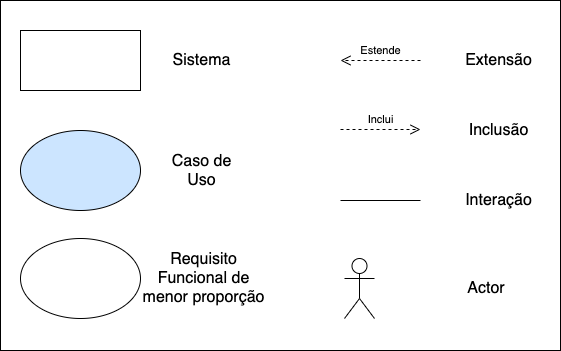
\includegraphics[width=0.7\textwidth]{img/rf/legenda}
		\caption{Legenda dos diagramas}
		\label{fig:rf-legenda}
	\end{center}
\end{figure}

Numa segunda fase serão analisados os graus de prioridade de cada requisito, consoante a sua importância para o projecto e por fim será feita uma descrição detalhada (i. e. especificação do requisito) de cada requisito através de casos de uso. É de notar que parte do grande trabalho da analise do grau de prioridade dos requisitos será imediato devido às decisões por parte do cliente.

Desta forma será claro para o leitor, em especial para a equipa de desenvolvimento, o comportamento que o sistema terá de cumprir. Os casos de uso serão detalhados consoante a seguindo estrutura:

\begin{itemize}
	\item \textbf{ID:} ID do caso de uso.
	\item \textbf{Ator:} Responsável pela realização do caso de uso.
	\item \textbf{Prioridade:} Representa a prioridade do caso de uso baseada nas decisões do cliente, visão dos stakeholders e no funcionamento do sistema. As prioridades foram classificadas por:
	\begin{itemize}
		\item \textbf{\textit{Must Have}:} Como o próprio nome indica, os requisitos \textit{Must} são os requisitos com maior prioridade. \textit{"As a rule, product inception depends entirely on defining must-haves using such pointers as ‘required for launch’, ‘required for safety’, ‘required for validation’, ‘required to deliver a viable solution’, etc."}\cite{moscow}. Todos os requisitos categorizados como \textit{Must Have}, são mandatórios para a equipa de desenvolvimento visto que sem eles o projecto fica paralisado.\textit{ "Can we move forward with the project if this task is undone? – if \textbf{NO}, it’s \textbf{MUST}"}\cite{moscow}.
		\item \textbf{\textit{Should Have}:} Os requisitos \textit{Sould} são requisitos que também têm uma elevada prioridade, ou por outras palavras, estão apenas um passo a baixo dos requisitos \textit{Must} .
		Não são requisitos considerados vitais contudo adicionam valor significativo.\textit{ "Will we move forward with the project if this task is done a bit later? – if \textbf{YES}, it’s \textbf{SHOULD}"}\cite{moscow}.
		\item \textbf{\textit{Could Have}:}\textit{ "Can we sacrifice this task till deadline? – if \textbf{YES}, it’s \textbf{COULD}"}\cite{moscow}.
		\item \textbf{\textit{Won't Have}:}\textit{ "Can we back to it when things go better? – if \textbf{YES}, it’s \textbf{WON’T}"}\cite{moscow}.
	\end{itemize}
	\item \textbf{Descrição:} Uma breve contextualização do caso de uso.
	\item \textbf{Pré-condições:} Conjunto de condições necessárias para realizar o caso de uso.
	\item \textbf{Estimulo:} Casos de uso responsáveis pela ativação do caso de uso.
	\item \textbf{Fluxo Principal:} Descrição detalhada de todos os passos para a realização do casos de uso.
	\item \textbf{Fluso de Excepção:} Descrição detalhada do comportamento do sistema quando o caso de uso não for realizado com sucesso.
	\item \textbf{Observações:} Observações adicionais, relevantes para o desfecho do caso de uso.
\end{itemize}

\newpage

\subsection{Diagrama de contexto}
\label{d:contexto}
\begin{figure}[ht!]
	\begin{center}
		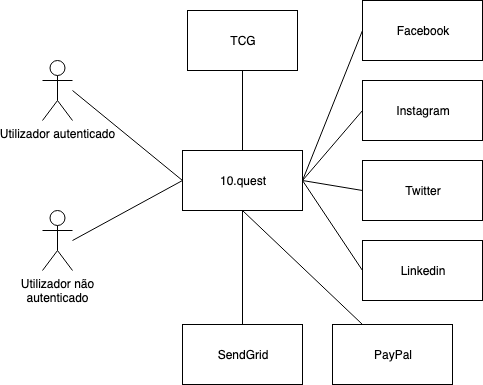
\includegraphics[width=0.6\textwidth]{img/rf/10quest}
		\caption{Diagrama de contexto}
		\label{fig:rf-10quest}
	\end{center}
\end{figure}

A 10.quest, tal como referido nos capítulos anteriores, é uma plataforma de inbound marketing que permite aos utilizadores criar formações, questionários, concursos e tratar a informação recolhida por cada um destes componentes. 
Estes componentes poderão ser partilhados nas redes sociais (i. e. utilizando a API do Facebook, Instragam, Twitter e LinkedIn) através de \textit{landing pages}. Estas \textit{landing pages} terão um pequeno formulário que necessita das informações básicas ao utilizador final para que, automáticamente, as formações, questionários e concursos sejam enviados por mail para os inscritos, utilizando o sistema externo SendGrid.

Tal como referido no Capítulo \ref{sec:estado-arte}, o \acrshort{tcg} é um produto desenvolvido pela 10.digital e actualmente no mercado. Algumas das funcionalidades fundamentais da plataforma a desenvolver já estão implementadas no \acrshort{tcg}  e por isso mesmo haverá uma interação com o mesmo para aproveitar todas estas funcionalidades necessárias.


\newpage

\subsection{Diagrama de alto nível}
\label{d:altonivel}
\begin{figure}[ht!]
	\begin{center}
		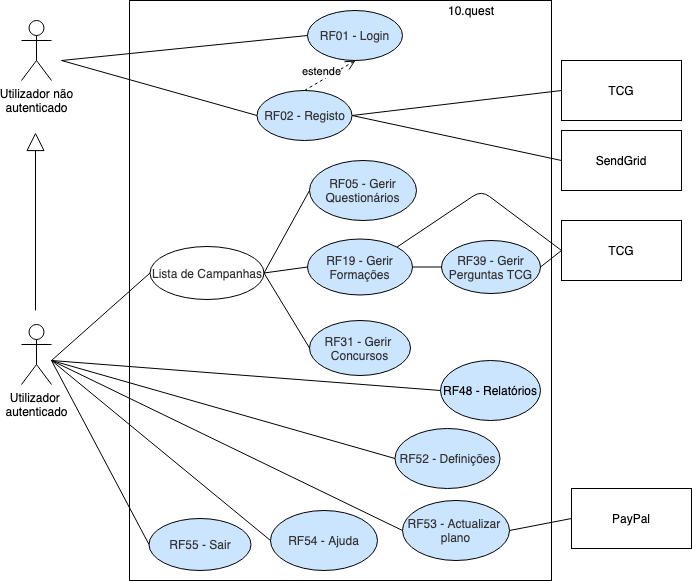
\includegraphics[width=0.8\textwidth]{img/rf/alto-nivel}
		\caption{Diagrama de Alto Nível}
		\label{fig:rf-alto-nivel}
	\end{center}
\end{figure}

Um utilizador para aceder a todas as funcionalidades da plataforma terá de primeiro realizar a autenticação através do caso de uso \textbf{RF - Registo}. Caso ainda não tenha uma conta registada terá de o fazer. Assim que a conta for criada é enviada uma notificação para o email do utilizador, recorrendo ao sistema externo SendGrid. Por questões de segunrança e confidencialidade dos dados, no acto do registo, a informação do utilizador será enviada e guardada na base de dados do \acrshort{tcg}, para que mais tarde todos os pedidos REST possam ser validados.

Depois de um utilizador se autenticar, será direcionado para a página inicial. A partir daqui o utilizador conseguirá gerir questionários, formações, concuros e perguntas para as formações do \acrshort{tcg}; aceder às definições, actualizar o plano da conta, utilizar o suporte da plataforma e terminar sessão.
Ainda na página inicial da plataforma serão exibidas algumas estatísticas relacionadas com as formações, questionários e concursos associados à conta do utilizador. 

\newpage

\subsection{Diagrama Registo}
\label{d:registo}
\begin{figure}[ht!]
	\begin{center}
		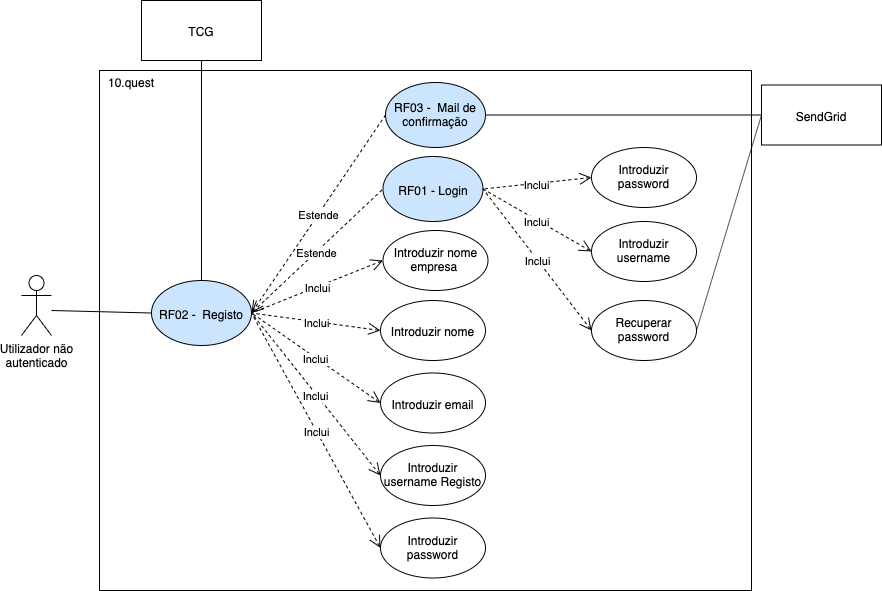
\includegraphics[width=1\textwidth]{img/rf/registo}
		\caption{Diagrama Gerir Concursos}
		\label{fig:rf-registo}
	\end{center}
\end{figure}

Para se efectuar um registo é necessário introduzir o nome da empresa, nome do utilizador, email, \textit{username} e \textit{password}. De seguida o utilizador é direcionado para a página de login onde terá de introduzir o \textit{username} e \textit{password} para se autenticar.

Depois de se efectuar um registo é enviado um mail de confirmação para o email associado à conta.

\newpage

\subsection{Diagrama Gerir Perguntas TCG}
\label{d:perguntastcg}
\begin{figure}[ht!]
	\begin{center}
		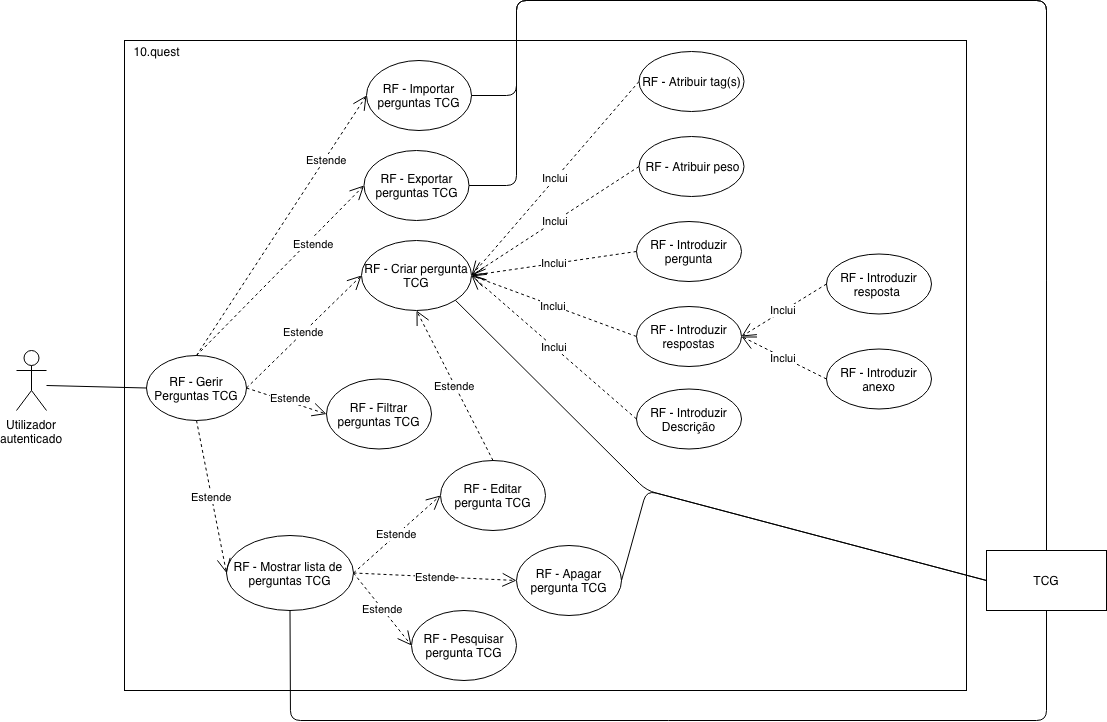
\includegraphics[width=1\textwidth]{img/rf/gerir-perguntas-tcg}
		\caption{Diagrama Gerir Perguntas TCG}
		\label{fig:rf-gerir-perguntas-tcg}
	\end{center}
\end{figure}

No \acrshort{tcg}, tal como referido no Capítulo \ref{sec:TCG}, a criação de questões é isolada da criação de formulários. Dito isto é necessário criar questões para que se possa ter conteúdos para as formações. 

Aproveitando as funcionalidades do \acrshort{tcg} e  tendo em conta que esta abordagem traz uma serie de vantagens, referidas no Capítulo \ref{sec:TCG}, a plataforma a desenvolver irá seguir o mesmo modelo. 

É ainda de notar que por uma questão de terminologia, na plataforma a desenvolver, as Perguntas TCG são equivalentes às questões no \acrshort{tcg}, pelo simples facto de não se confundir com elementos relacionados com os questionários.

Na gestão de Perguntas TCG, um utilizador consegue listas todas as perguntas associadas à sua conta (i. e. criadas por ele) e pode também criar uma nova pergunta. O sistema efetua um pedido de todas essas perguntas ao \acrshort{tcg} e a partir daqui o utilizador consegue criar, eliminar, editar e pesquisarperguntas. As perguntas podem também ser importados e exportados através de uma \textit{spreadsheet}.

Para um criar uma pergunta, o utilizador precisa de atribuir uma tag, nova ou existente, e introduzir a pergunta, as respotas e umas descrição, sendo esta ultima opcional. Cada pergunta tem que ter pelos menos duas respostas sendo estas compostas pela resposta e um anexo opcional que pode ser um ficheiro de som, imagem ou vídeo.



\newpage

\subsection{Diagrama Gerir Formações}
\label{d:formacoes}
\begin{figure}[ht!]
	\begin{center}
		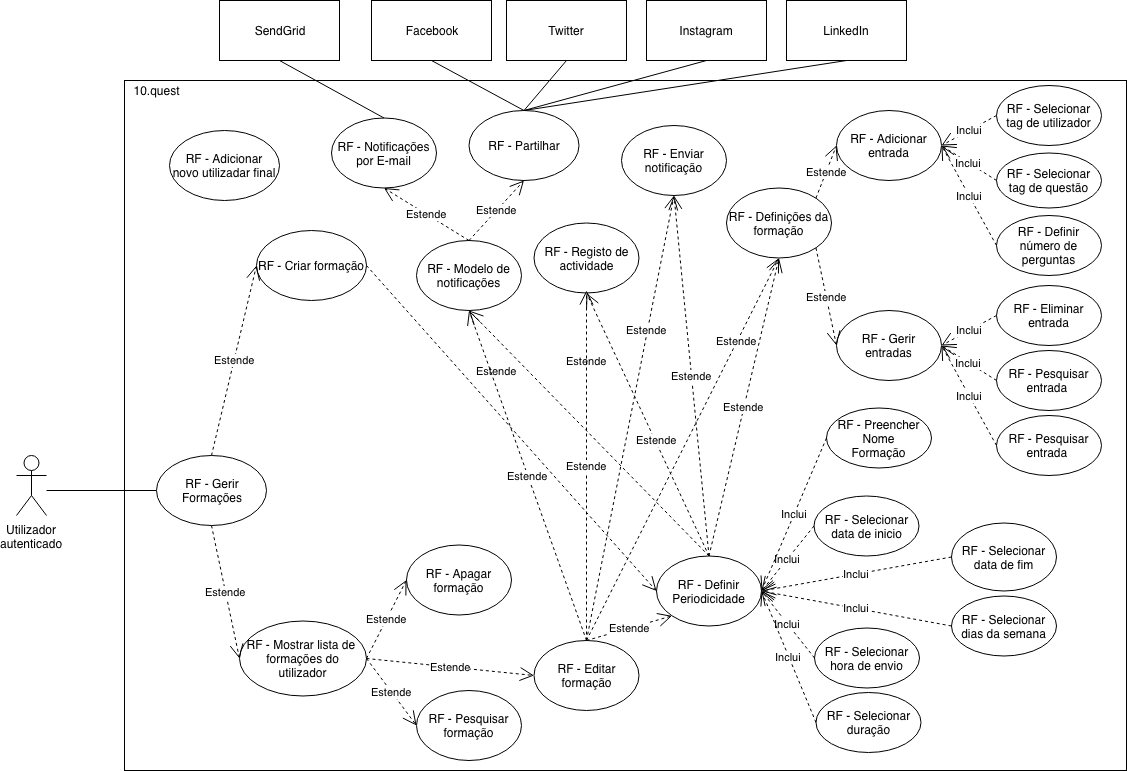
\includegraphics[width=1\textwidth]{img/rf/gerir-formacoes}
		\caption{Diagrama Gerir Formações}
		\label{fig:rf-gerir-formacoes}
	\end{center}
\end{figure}

Praticamente todas as funcionalidades da gestão de formações já estão implementadas no \acrshort{tcg} por isso, muitas das funcionalidades irão recurar a à capacidade do \acrshort{tcg} através de pedidos REST e toda a informação relacionada com formações será também guardada na bade de dados do \acrshort{tcg}.

Na gestão de formações um utilizador consegue listar todas as formações associadas à sua conta e pode também criar uma nova formação. O sistema efetua um pedido de todas essas formações ao \acrshort{tcg} e a partir daqui o utilizador consegue criar, eliminar, editar e pesquisar formações.

Para criar uma formação o utilizador terá, numa primeira instância, de atribuir um nome e definir a periodicidade (i. e. preencher a data de inicio e fim, dias da semana, hora de envio e  duração/validade). 

Numa segunda fase, o utilizador, através do requisito \textbf{RF - Definições da formação} consegue adicionar e gerir entradas. As definições da formação é onde o utilizar, através de \textit{tags} associa grupos de perguntas a grupos de pessoas. 

Numa entrada o utilizador terá de introduzir a \textit{tag} de utilizador(es), a \textit{tag} da(s) pergunta(s) e o número de perguntas dessa \textit{tag} que serão enviadas em cada \textit{quiz}(i. e. cada iteração) da formação.

Por fim o utilizador pode partilhar a formação. As inscrições numa formação serão feitas através de uma \textit{landing page} que pode ser personalizada no requisito \textbf{RF - Partilhar} e enviadas para o email introduzido no mini formulário da \textit{landing page}. Este mail com o link para a formação, pode ser persolizado no requisito \textbf{RF - Notificações por E-mail}. 

É de notar que, através do resquisito \textbf{RF - Adicionar novo utilizador final TCG}, sempre que um utilizador final se inscreve numa formação através da \textit{landing page}, o sistema, de forma automática, envia os dados para \acrshort{tcg} para que este utilizador possa começar a receber a formação por email. Outro requisito da responsabilidade do sistema é o \textbf{RF - Notificar utilizadores finais TCG}, que respeitando a peridicidade definida na criação do formação, envia a formação para todos os inscritos.



\subsection{Diagrama Gerir Questionários}
\label{d:quests}
\begin{figure}[ht!]
	\begin{center}
		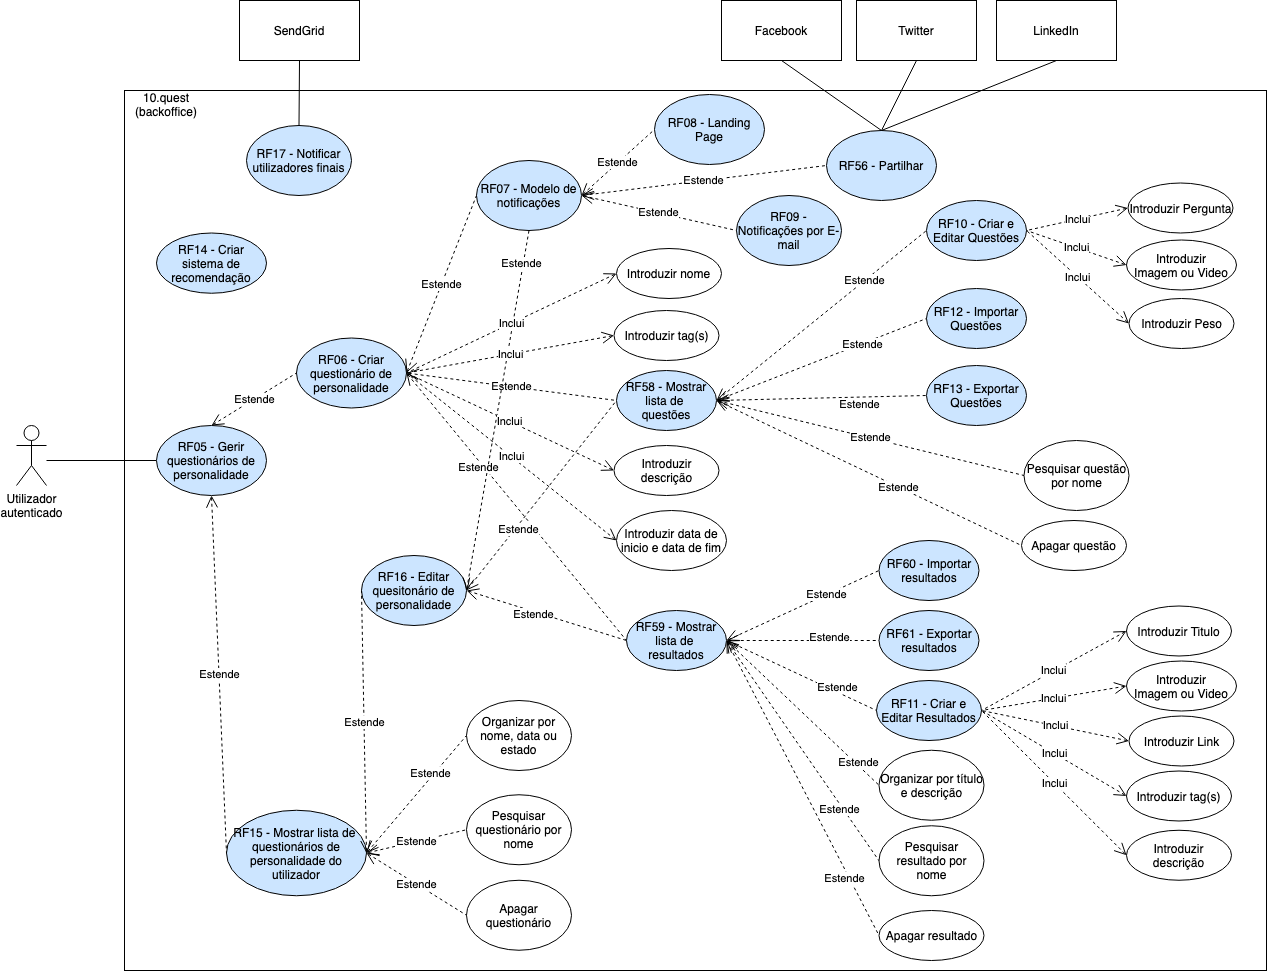
\includegraphics[width=1\textwidth]{img/rf/gerir-quest}
		\caption{Diagrama Gerir Questionários}
		\label{fig:rf-gerir-quest}
	\end{center}
\end{figure}

Na gestão de questionários, à semelhança da gestão de formações, é feita uma listagens dos questionários e o utilizador tem a capacidade de criar, eliminhar, editar e pesquisar questionários.

Na criação de um novo questionário, um utilizador, numa primeira fase 
terá de criar um contundo de perguntas e gerar um serie de resultados. Cada resultado terá de ter obrigatóriamente uma \textit{tag} associada e um título e caso o utilizador deseje uma imagem e/ou um link. As perguntas e resultados podem também ser importados e exportados numa \textit{spreadsheet}.

Depois de terminar a primeira fase, podendo a qualquer momento voltar a essa fase, o utilizador já tem recursos para começar a criar o quesitonário (i. e. o sistema de pontuação através do requisito \textbf{RF - Criar sistema de pontuação}). Numa primeira instancia o utilizador terá de selecionar a pergunta pelo qual deseja começar o questionário. De seguida cria uma ou mais respostas e para cada uma delas é necessário associar uma pergunta que na iteração seguinte sejam apresentadas e se possa repetir este processo para conseguir criar um fluxo de perguntas. Para cada pergunta é atribuido um peso e para cada resposta são associadas \textit{tags} de resultados. Desta forma numa dada pergunta, as \textit{tags} da resposta selecionada serão pontuadas.
 A qualquer momento o utilizador, em vez de associar uma pergunta a uma resposta, pode decidir, naquele estado (i. e. numa resposta em especifico), terminar o questionário e apresentar o resultado ao utilizador final. 

Através do requisito \textbf{RF - Adicionar novo utilizador final}, sempre que um utilizador final se inscreve num questionário através da \textit{landing page}, o sistema, de forma automática, guarda essa informação e recorrendo ao requisito \textbf{RF - Notificar utilizadores finais}, enviei o questionário para os utilizador final.


\subsection{Diagrama Gerir Concursos}
\label{d:concursos}
\begin{figure}[ht!]
	\begin{center}
		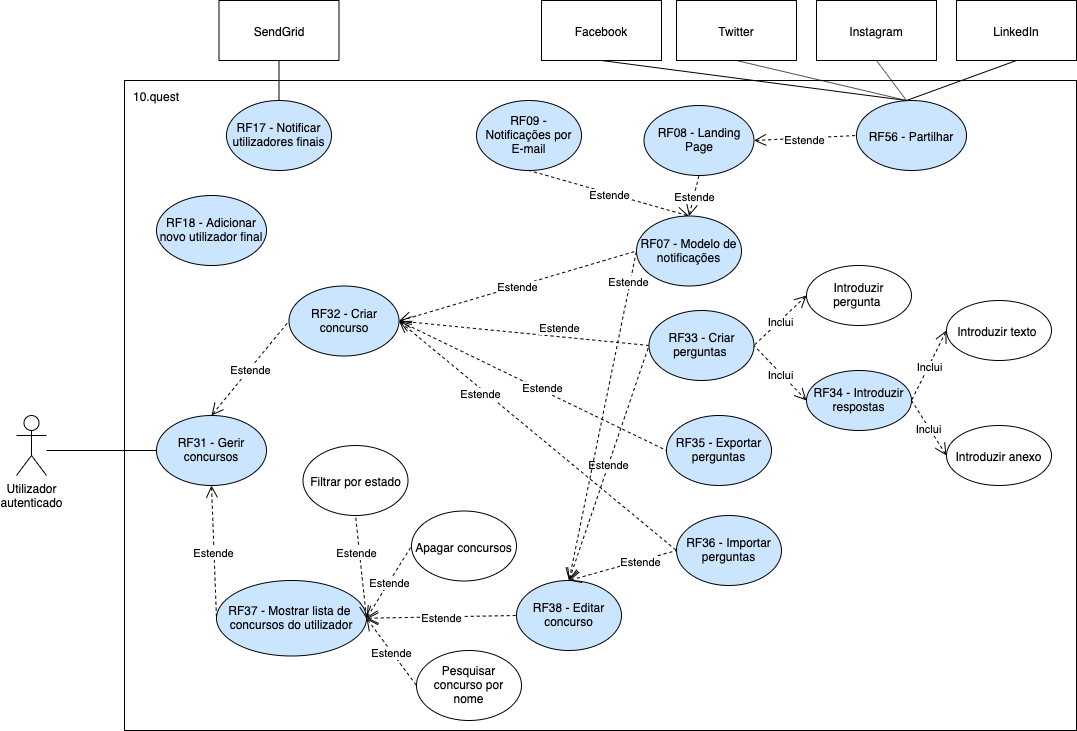
\includegraphics[width=1\textwidth]{img/rf/gerir-concurso}
		\caption{Diagrama Gerir Concursos}
		\label{fig:rf-gerir-concursos}
	\end{center}
\end{figure}


Na gestão de concursos, à semelhança da gestão de formações e questionários, é feita uma listagens dos concursos e o utilizador tem a capacidade de criar, eliminhar, editar e pesquisar questionários.

Na criação de um concursos o utilizador terá de criar perguntas. Para cada pergunta o utilizador terá de introduzir pelo menos duas respostas e caso o desejo pode adicionar um anexo no formato de imagem. As perguntas e respostas podem também ser importados e exportados numa \textit{spreadsheet}.

É importante referenciar que à semelhança da gestão de formações e questionários, é possível editar os conteudos (i. e. perguntas, questões, \textit{landing pages}, email etc) contudo, assim que um concurso é publicado e passa a estar no estado \textit{online}, as perguntas deixam de poder ser editaveis. 

Os concursos, tal como os questionários têm sempre um estado que pode variar entre:
\begin{itemize}
	\item Rascunho - Utilizador não deu o concurso como conluído.
	\item Aberto - Utilizador deu o concurso como conluído.
	\item \textit{Online} - Utilizador gerou a \textit{landing page} para partilhar o concurso.
	\item Fechado - Concurso chegou à data de fim.
\end{itemize}


\subsection{Diagrama Ajuda}
\label{d:ajuda}
\begin{figure}[ht!]
	\begin{center}
		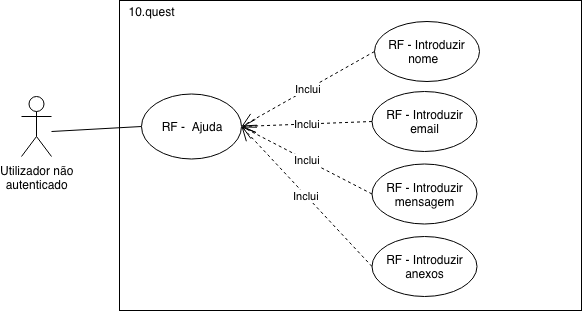
\includegraphics[width=1\textwidth]{img/rf/ajuda}
		\caption{Diagrama Ajuda}
		\label{fig:rf-ajuda}
	\end{center}
\end{figure}


O utilizar poderá, se assim o pretender, utilizar o suporte da plataforma. Em caso de dúvida ou exclarecimentos, enviar uma mensagem directa para a 10.digital. 

Para enviar uma mensagem é necessário introduzir o nome, email, mensagem e, caso o utilizador deseje, um ou mais anexos.



\newpage
\section{Prototipagem}
\label{prototipagem}


%-------------------------------------------------------------------------------------------------
\blankpage
%-------------------------------------------------------------------------------------------------

\glsresetall